\documentclass[12pt, a4paper, oneside]{article}
\usepackage{amsmath, amsthm, amssymb, graphicx}
\usepackage[bookmarks=true, colorlinks, citecolor=blue, linkcolor=black]{hyperref}
\usepackage[margin = 25mm]{geometry}
\usepackage{setspace}
\usepackage{graphicx}

% introductory area
\title{The renaissance of jet physics report}
\date{\today}
\author{202011010101 Physics 2001 Sun Tao'an}
\begin{document}
\begin{spacing}{2.0}
\maketitle
\section{introduction}
This paper mainly studies the content of Mr. Zhongbo Kang's speech at Hunan University on 2022/06/20, that is, the research on jet.
In a high-energy particle collider, two (or more) particles collide and move in a specific direction, and the reflected particles are usually gluons or quarks.
The jet is created during QCD scattering, producing high lateral momentum quarks or gluons. The probability of producing a particular jet is described by the jet production cross section,
It is an average of fundamental perturbative QCD quark, antiquark, and gluon processes, weighted by a partial distribution function.
For the most frequent jet pair generation process, i.e. the scattering of two particles, the jet generation cross section in hadron collision is given by
$\sigma_{i j \rightarrow k}=\sum_{i, j} \int d x_{1} d x_{2} d \hat{t} f_{i}^{1}\left(x_{1} , Q^{2}\right) f_{j}^{2}\left(x_{2}, Q^{2}\right) \frac{d \hat{\sigma}_{i j \rightarrow k} }{d \hat{t}}$\\
$x, Q^2$: Longitudinal momentum components and momentum transfer\\
$\hat{\sigma}_{i j \rightarrow k}$: Perturbative QCD cross section of reaction ij → k\\
$f_{i}^{a}\left(x_{a}, Q^{2}\right)$: The partial subdistribution function used to find particle species i in beam a. \\
Perturbative QCD calculations may have a colored part in the final state, but only the final produced colorless hadrons are observed experimentally.
Therefore, to describe what is observed in the detector as a result of a given process, all colored parts of the output must first undergo partial sub-showers,
The resulting parts are then combined into hadrons. The terms fragmentation and hadronization are often used interchangeably in the literature to describe soft QCD radiation, hadron formation,
Or use both processes at the same time.
Due to the partial exit interaction created in hard scattering, the strong coupling constant will increase with its separation.
This increases the probability of QCD radiation, which is mainly at shallow angles relative to the original part. Thus, one segment radiates gluons, which in turn radiate "$\bar{qq}$" pairs, with each new segment nearly collinear with its parent.

\section{Begining of jet physics}
The study of jets is very early, George Strman published "Jets from Quantum Chromodynamics"\cite{PhysRevLett.39.1436} in 1977,
It is mainly that the collisions of $e^+$ and $e^-$ reflect quarks (back to back) in both directions. \\
And also around 1979, "Search for gluons in $e^+e^-$ annihilation"\cite{ELLIS1976253} found gluons in a similar way,
When the energy is large enough, the quarks in the final state may separate gluons.

\begin{figure}[htbp]
\centering
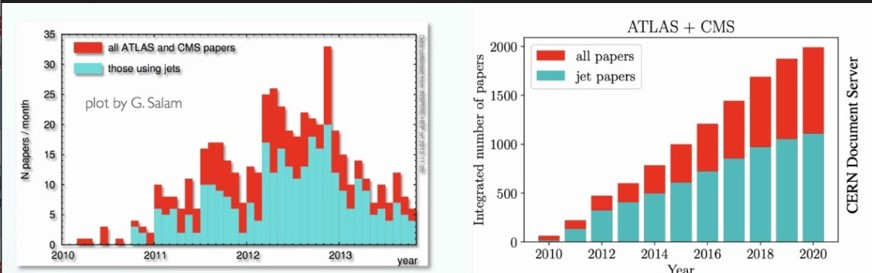
\includegraphics[width=8cm]{sigma.jpg}
\caption{statistics graph 1 by report}
\end{figure}
\subsection{What are we using jets for?}
\subsubsection{Quantum imaging of protons and nuclei}
Just as black hole imaging shows gravitational dynamics, proton imaging will provide insights into the strong interaction, especially on the momentum scale corresponding to the size of the proton,
Analysis of particle spins by 3D imaging may also have a role in MRI.
Subatomic particles have the quantum mechanical property of spin. Certain nuclei, such as 1H (proton), 2H, 3He, 23Na, or 31P, have non-zero spin and therefore magnetic moments.
For so-called spin 1⁄2 nuclei, such as 1H, there are two spin states, sometimes called up and down.

When these spins are placed in a strong external magnetic field, they precess around the axis in the direction of the magnetic field. Protons are arranged in two energy eigenstates (the Zeeman effect):
One low energy and one high energy, which are separated by very small splitting energies.
\subsubsection{A New Glassy State of Matter: The Color Glass Condensate}
First, color charge is a property of quarks and gluons related to the strong interactions of particles in quantum chromodynamics (QCD) theory.
The "color charge" of quarks and gluons has absolutely nothing to do with the everyday meaning of color and charge. The terms color and red, green, and blue labels became popular simply because of loose analogies to primary colors.
Some particles have corresponding antiparticles. Particles with red, green, or blue charges have corresponding antiparticles, where the color charge must be the inverse of red, green, and blue, respectively,
in order to maintain color charge in particle-antiparticle creation and annihilation. Particle physicists call these anti-red, anti-green and anti-blue. All three colors mixed together,
Or any of these colors, and their complement (or negative), are "colorless" or "white" with a net color charge of zero. Due to a property of strong interactions called color confinement,
A free particle must have zero color charge: a baryon consists of three quarks, which must be one of red, green, and blue;
Likewise, an antibaryon consists of three antiquarks, one each of anti-red, anti-green, and anti-blue. A meson consists of a quark and an antiquark;
Quarks can be any color, and antiquarks have corresponding anticolors.
And jet physics can help observe the sixth state of colored glass condensates beyond solids, liquids, gases, plasmas, and Bose-Einstein condensates. \cite{https://doi.org/10.1111/ijag.12013}
\subsubsection{jet propagation in nuclear matter}
In heavy ion reactions, jets are widely used as probes in quark-gluon-plasma (QGP) studies.
The propagation of the jet in the medium also affects the measurements of strongly interacting nuclear matter properties.
This in turn affects the propagation and interaction of high-energy quarks and gluons in dense QCD matter. \cite{Ovanesyan_2011}
Theoretical study involving jet cross-section and jet charge
Electron-Ion Collider. predict these observables in electron gold relative to
Electron-proton collisions reveal how flexible centroid energies and motion coverage
The new facility could be used to boost the signal and maximize the impact of the electronic nuclear program.
At the same time, it can also be proved theoretically how to disentangle the influence of nucleon distribution\cite{PhysRevLett.126.252001}
\begin{figure}
    \begin{minipage}[t]{0.5\linewidth}
        \centering
        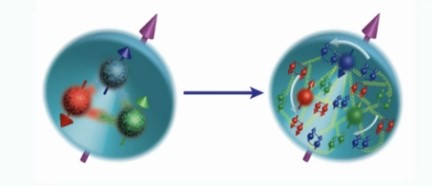
\includegraphics[scale=0.3]{kappa.jpg}
        \caption{Quantum imaging of protons and nuclei}
        \label{fig:side:a}
      \end{minipage}%
      \begin{minipage}[t]{0.5\linewidth}
        \centering
        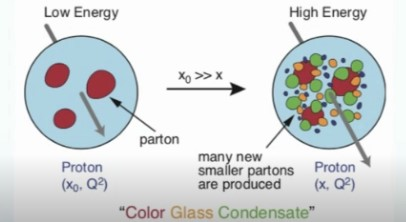
\includegraphics[scale=0.3]{mu.jpg}
        \caption{A new form of matter - color glass condensate}
        \label{fig:side:b}
      \end{minipage}
\end{figure}
\begin{figure}
    \centering
    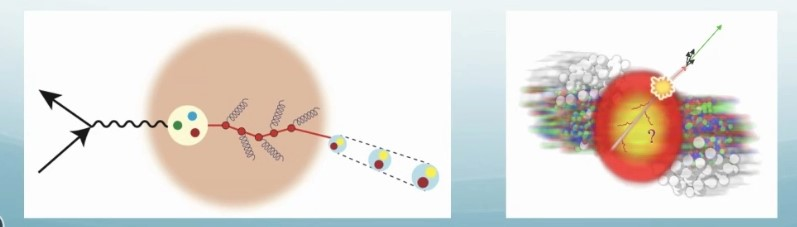
\includegraphics[width=8cm]{nu.jpg}
    \caption{jet propagation in muclear matter}
\end{figure}

\subsection{imaging a proton}
Studying the process of black holes leads us to discover gravitational waves, and studying protons allows us to discover the inner workings of strong interactions,
Our problem now is \\
(1) How the properties of nucleons such as mass and spin are generated from elementary quarks/gluons\
(2) Quantum correlation between quark spin and proton spin
\subsubsection{fundamental structure of proton?}
While protons were originally considered elementary particles, in the Standard Model of modern particle physics, protons are now called composite particles containing three valence quarks and are now classified as hadrons along with neutrons.
According to the Standard Model, a proton consists of three quarks: two up and one down. These quarks combine to give it charge and spin.
The +1 charge of the proton comes from the combined charge of two up quarks ($+\frac{2}{3}$ each) and one down quark ($-\frac{1}{3}$). The three quarks are held together by a powerful force;
The energy of these bonds determines most of the mass of the proton. Because a proton consists of three quarks bound together, it is a baryon. Neutrons are also baryons, consisting of two down quarks and one up quark
, so there is no net charge.

\section{Connecting theory and experiment}
This part uses the work of phenomenology within the scope of the theory, from experimental data to obtain the connection of protons in terms of quarks, for Figure (a) can be designed experiments

\begin{figure}
    \centering
    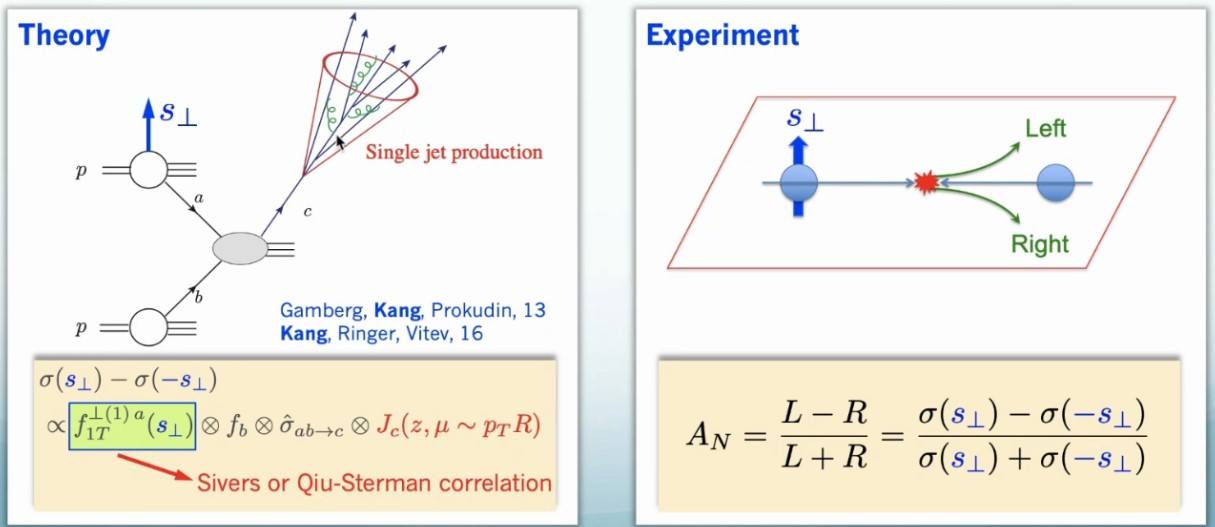
\includegraphics[width=8cm]{theory and experiment.jpg}
    \caption{the comparison of theory and experiment}
\end{figure}


%This is very important and must be expanded!!!!!
\subsection{Experiment introduce}
Two protons can interact and their final state will produce a jet. At this time, we can try to detect the correlation we need for a proton, and observe each particle to construct several relations.
This section uses the work of phenomenology within the theoretical context, so that we only need to compare with experimental data.
But we can find that for single jet, his momentum is about 60GeV-100GeV, and our associated lateral momentum is about 1GeV, so we can't observe,
In this regard, the experimental method can be improved,
Small lateral momentums such as the imbalance of lateral momentum ($q_T$) in the dijet are further measured experimentally (see Figure b) to construct a valid field theory
\begin{figure}
    \centering
    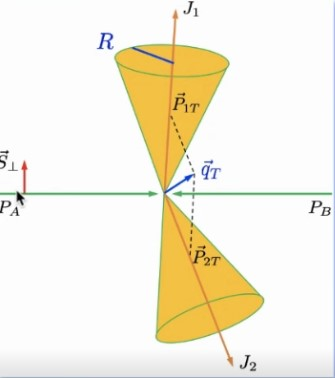
\includegraphics[width=8cm]{delta.jpg}
    \caption{Improvements to experiments}
\end{figure}

\subsection{Experiment data}
We can see from the experimental data that the data of either singlejet or dijet are very close to 0.

\begin{figure}
    \begin{minipage}[t]{0.5\linewidth}
        \centering
        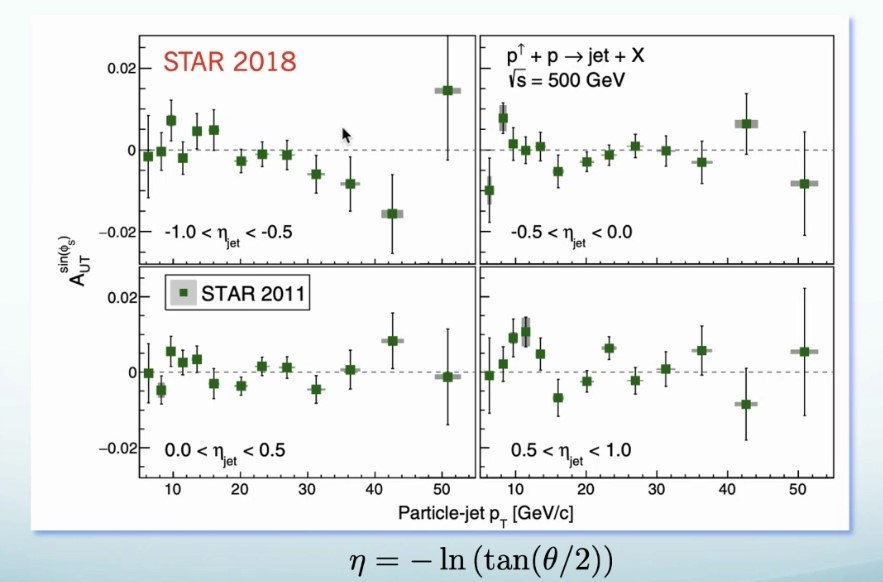
\includegraphics[scale=0.3]{alpha.jpg}
        \caption{singlejet}
        \label{fig:side:a}
      \end{minipage}%
      \begin{minipage}[t]{0.5\linewidth}
        \centering
        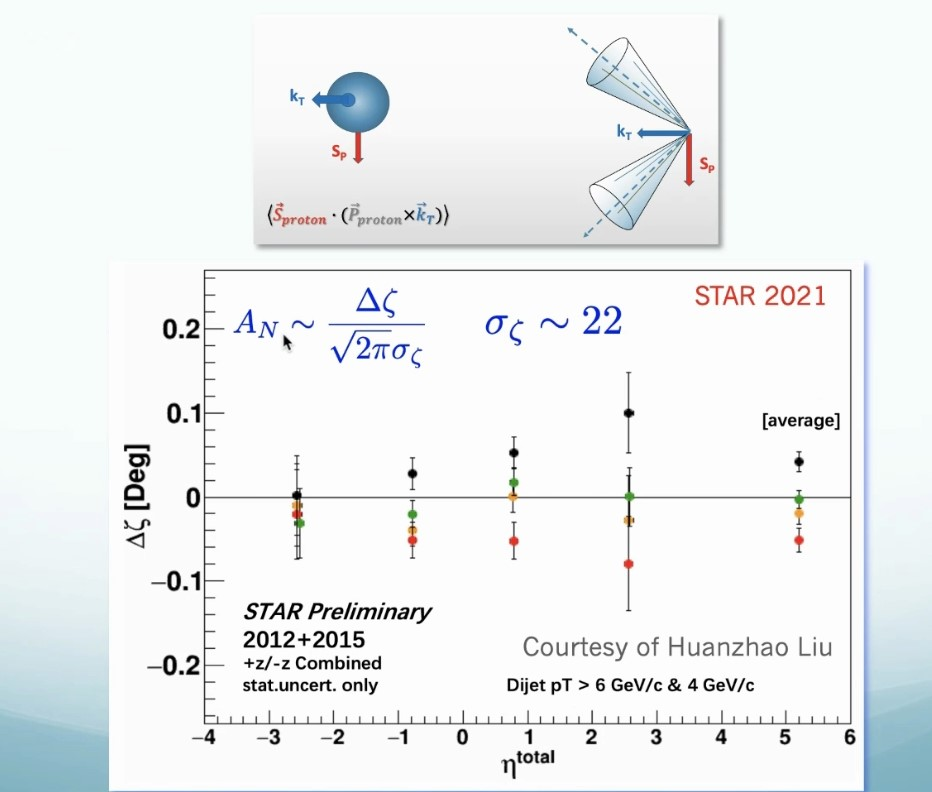
\includegraphics[scale=0.3]{dijet.jpg}
        \caption{dijet}
        \label{fig:side:b}
      \end{minipage}
 
\end{figure}
But this does not mean that quantum relationships do not exist, in fact we can first try to see the measurement of hadron interactions, we use two ways: SIDIS and Drell-Yan
Then the final result of collecting the data can be seen to be symmetrical, but at present we cannot distinguish the jets generated by u quark and d quark in the picture whether we are using single jet or dijet,
So for now we can only add them all up, which is why we don't see symmetry.
So we introduce Aharonov-Bohm effect below to solve this problem

\begin{figure}
    \begin{minipage}[t]{0.5\linewidth}
        \centering
        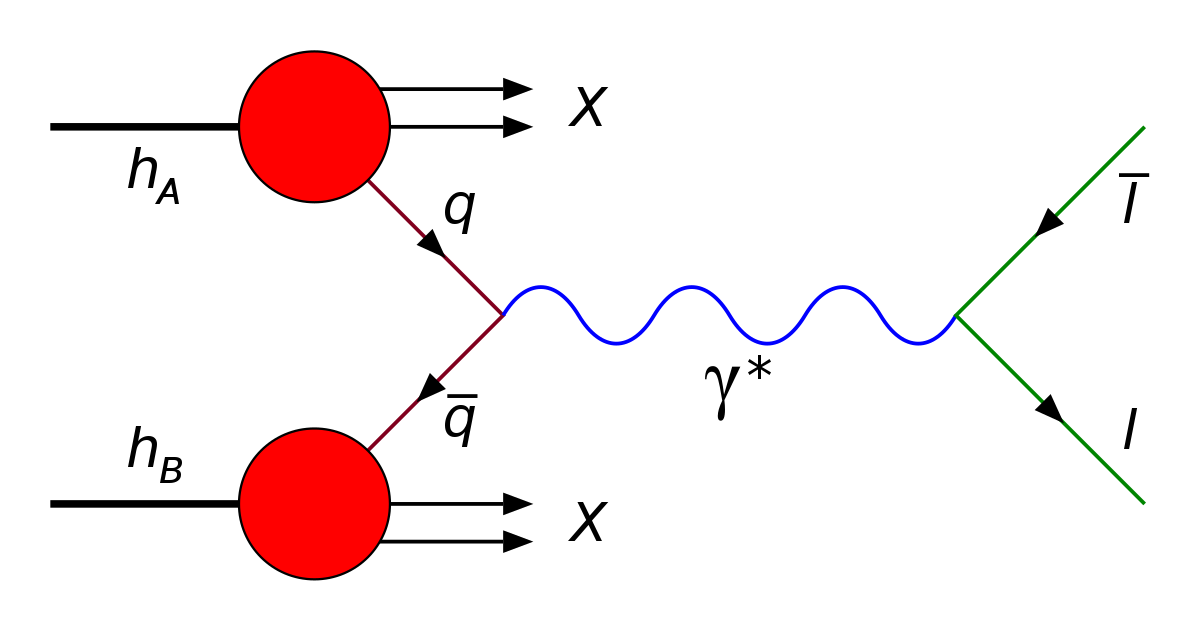
\includegraphics[scale=0.1]{drellyan.png}
        \caption{Drell-Yan}
        \label{fig:side:a}
      \end{minipage}%
      \begin{minipage}[t]{0.5\linewidth}
        \centering
        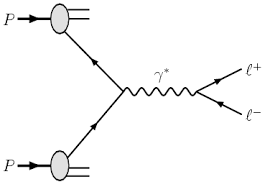
\includegraphics[scale=0.3]{SIDIS.png}
        \caption{SIDIS}
        \label{fig:side:b}
      \end{minipage}
\end{figure}
\begin{figure}
    \centering
    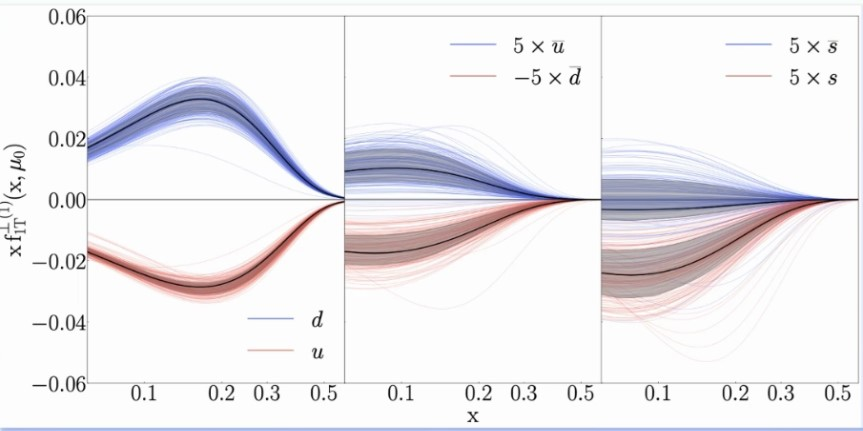
\includegraphics[width=8cm]{theta.jpg}
    \caption{asymmetry}
\end{figure}


\subsection{Quantum phase:akin Aharonov-Bohm effect}
The Aharonov-Bohm effect is a quantum mechanical phenomenon in which charged particles are subjected to an electromagnetic potential ($\phi$, A), although they are confined to a region where the magnetic field B and electric field E are zero.
The basic mechanism is the complex-phase coupling of the electromagnetic potential and the charged particle wave function, and the interference experiment correspondingly illustrates the Akhalonoff-Bohm effect.

The Aharonov-Bohm effect is conceptually important because it involves three obvious problems of recasting (Maxwell's) classical electromagnetic theory into gauge theory,
Before quantum mechanics, it could be thought of as a mathematical reconstruction without physical consequences.
The three questions are:
Whether potential energy is "physical" or just a handy tool for calculating force fields;
Whether the principles of action are basic;
locality principle.
The Aharonov-Bohm effect proves that even in the region of zero magnetic field, the magnetic effect still exists, however, this cannot be used to measure the magnetic vector potential, because only the magnetic flux will appear in the formula expressing the effect,
And the whole theory always maintains norm invariance. The Akhanov-Bohm effect is an important experiment in the development history of quantum mechanics and electrodynamics, which illustrates the non-local nature of quantum mechanics.
Applied to our jet, $e^{i\phi}$$\phi = g_s \int_{path} \mathrm{d r}\cdot A$ for DIS quark passing through reman's gauge field to produce phase rotation
, and because the two passes on the optical cone are different, through such different phases, it can be proved that $Sivers function|_{DIS} = -Sivers function|_{DY}$


\begin{figure}
    \begin{minipage}[t]{0.5\linewidth}
        \centering
        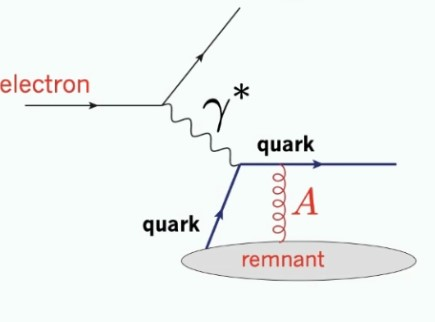
\includegraphics[scale=0.1]{DIS.jpg}
        \caption{DIS}
        \label{fig:side:a}
      \end{minipage}%
      \begin{minipage}[t]{0.5\linewidth}
        \centering
        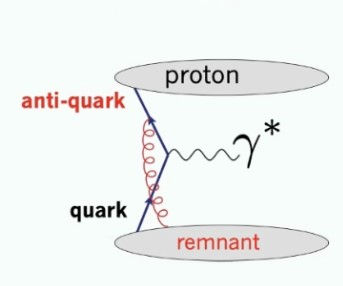
\includegraphics[scale=0.3]{drell.jpg}
        \caption{drell-yan}
        \label{fig:side:b}
      \end{minipage}
\end{figure}

And the association between these "Sivers" can affect our classification of u quark and d quark

\section{separate the quarks}

%idea:u and d have different charges, u quark have $+\frac{2}{3}e$, and the d quark have $-\frac{1}{3}e$
%if we can sum all the charge where in the end of the jet, we probabily can separate the u quark and d quark
We have a conjecture for separating u quark and d quark: because u quark($+\frac{2}{3}e$) and d quark($-\frac{1}{3}e$) have different charges
, so if we can add up all the jet's end-charges, we can potentially separate u quark and d quark.
Total charge $Q_k \equiv \sum_{h\in jet}z^{\kappa}_hQ_h$, $z_h = \frac{p_{hT}}{p_{jT}},\kappa = 0.3,0.4,\ dots,1.0$
\begin{figure}
    \centering
    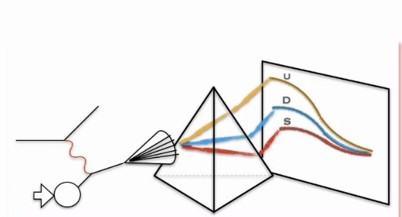
\includegraphics[width=8cm]{gamma.jpg}
    \caption{to get started, we decide to first look at jet production at the EIC}
\end{figure}
\begin{figure}
    \centering
    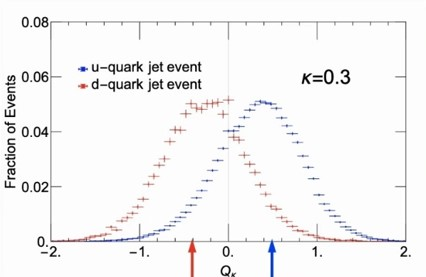
\includegraphics[width=8cm]{xi.jpg}
    \caption{jet charge distribution of u and d jets}
\end{figure}
\begin{figure}
    \centering
    
\includegraphics[width=8cm]{omega.jpg}
    \caption{organize the cross section via jet charge bin}
\end{figure}
No Emission Charge Option: d-quark removed, little change, so no sensitivity
Negative Emission Charge Vessel Option: Higher Sensitivity
The jet example shows. Studying the composition inside the jet can give you new insights into the jet substructure,
Help us achieve goals that are otherwise unattainable.
 3D imaging of protons: Proton → quark/gluon distribution partial distribution n• Hadronization:
Quark/gluon → hadron fragmentation function
This theoretical framework • is called polarized jet.



In particle physics, you generally don't care about the structure of the jet, because you just want to find particles beyond the standard model
The reason for paying attention to QCD is that when the momentum generated by particles beyond the standard model is small, their decay product will be large, and as the initial dynamic momentum increases, their included angle will become smaller and smaller,
There will be a jet called boosted partical


\section{Conclusion}
This report first introduces the reasons for the generation of jets and the substances that will be generated (generally gluons or quarks). The jets are generated during the QCD scattering process.
Generate high lateral momentum quarks or gluons. A perturbative QCD calculation may have a colored part in the final state, but only the final achromatic hadrons are produced by the real
observed experimentally.
The application examples of jet physics are also interspersed, and the theoretical innovations of many scholars in different directions are also introduced, including proton imaging, sixth-state colored glass condensates, etc.
Then briefly introduce jet and enter the planning experiment part. Here we will interact with two protons and their final state will produce a jet. At this time, we can try to test a
Protons detect the correlation we need, and observe each particle to construct several relations. This part is in the theoretical scope.
The phenomenological work is used within the scope, so that we only need to compare with experimental data.
However, it is found that the inadequacy of the Charity experiment will lead to the failure of the observation. In this regard, we improve the experimental method and further measure the small
Lateral momentum, such as the imbalance of lateral momentum in the dijet (see Figure b), thus constructs a valid field theory.
We followed two approaches separately: SIDIS and Drell-Yan and then collected the data.
But at present, we can't distinguish u quark and d in the picture whether we are using single jet or dijet
The jet produced by quark. Therefore, the Aharonov-Bohm effect was introduced and attempted to solve the problem.
For DIS quark to pass through reman's gauge field to produce phase rotation, $e^{i\phi}$$\phi = g_s \int_{path} \mathrm{d r}\cdot A$
, and because the two passes on the optical cone are different, through such different phases, it can be proved that $Sivers function|_{DIS} = -Sivers function|_{DY}$
This separates the quarks mentioned earlier.
The main method is to use the charge of quarks and pass the total charge of $Q_k \equiv \sum_{h\in jet}z^{\kappa}_hQ_h$, $z_h = \frac{p_{hT}}{p_{jT }},\kappa = 0.3,0.4,\dots,1.0$
At this point, the previous task can be completed.



\end{spacing}

\bibliographystyle{IEEEtran}
\bibliography{jet}



\end{document}